\documentclass[11pt,a4paper]{article}

\usepackage[utf8]{inputenc}
\usepackage[T1]{fontenc}
\usepackage[french]{babel}
\usepackage{amsmath,amssymb}
\usepackage{graphicx}
\usepackage[a4paper,margin=2.5cm]{geometry}
\usepackage{hyperref}
\hypersetup{colorlinks=true,linkcolor=black,urlcolor=blue,citecolor=black}

% Mise en page un peu plus aeree : interligne et espacement entre paragraphes.
\linespread{1.05}
\setlength{\parskip}{0.6em}

\graphicspath{{figures/}}

\title{Projet Méthodes Stochastiques\\[0.3em]
       \large Modèle proie-prédateur avec virus}
\author{Philippe \textsc{Lin} \and Sayna \textsc{Ren} \and Xuhong \textsc{Liu}}
\date{}

\begin{document}

\maketitle

\textit{Tous les résultats présentés dans ce rapport sont reproductibles dans le notebook qui l'accompagne, où l'on trouve également l'ensemble des codes.}

\section*{Contexte et modèle}

On étudie la dynamique de deux populations en interaction, les victimes (les proies) de densité $V_t$ et les prédateurs de densité $P_t$. Le point de départ est le modèle de Lotka-Volterra où les proies se reproduisent seules mais se font manger par les prédateurs tandis que les prédateurs meurent naturellement mais profitent de l'abondance des proies pour se reproduire.

Lorsqu'aucune perturbation extérieure n'intervient, cette dynamique s'écrit comme un système de Lotka-Volterra déterministe, avec $a$, $b$, $c$ et $d$ des coefficients positifs.

\begin{equation}\label{eq:base}
  dV_t = V_t\left(a - b\,P_t\right)dt,
  \qquad
  dP_t = P_t\left(-c + d\,V_t\right)dt.
\end{equation}

Un tel système admet des solutions périodiques si bien que les deux populations oscillent indéfiniment autour de leur point d'équilibre.

\section*{Question 1 — Proposer et valider un modèle pour le virus}

Dans le jeu de données \texttt{virus4.csv}, les proies sont en plus frappées par un virus que l'on modélise par un processus stochastique $(X_t)_{t\in[0,\tau]}$. Le système devient alors

\begin{equation}\label{eq:systeme}
  dV_t = V_t\left(\tfrac{2}{3} - \tfrac{4}{3}P_t + X_t\right)dt,
  \qquad
  dP_t = P_t\left(-1 + V_t\right)dt.
\end{equation}

Le fichier fournit une observation discrétisée de cette dynamique dont la première colonne correspond à $V_t$ et la seconde à $P_t$. Notre objectif est de proposer un modèle pour $(X_t)$ puis de le valider à l'aide de ces données.

Avant de nous lancer dans la modélisation, il nous a semblé naturel de commencer par regarder les données pour voir à quoi ressemblent les deux populations au cours du temps et en quoi elles s'écartent du modèle déterministe. Nous espérions ainsi nous faire une première idée de ce que le virus fait réellement au système.

\subsection*{Récupération du pas de temps}

Le fichier contient $2000$ points mais nous ne connaissions pas a priori le pas de temps de la discrétisation. Une idée a été d'exploiter le fait que l'équation des prédateurs ne contient aucun bruit puisque l'on a exactement $dP_t = P_t(-1 + V_t)\,dt$. En discrétisant, le pas de temps devrait alors vérifier

\begin{equation}\label{eq:dt}
  dt \approx \frac{P_{i+1} - P_i}{P_i\,(-1 + V_i)}.
\end{equation}

Nous avons donc moyenné cette quantité sur l'ensemble des points, en écartant ceux où le dénominateur $P_i(-1+V_i)$ est trop proche de zéro, soit que $V_i$ approche $1$, soit que $P_i$ approche $0$. Un seuil de $0{,}001$ sur $|P_i(-1+V_i)|$ ne retire qu'environ $4\,\%$ des points et donne $dt \approx 0{,}015$, soit une durée d'observation $\tau = 2000 \times 0{,}015 = 30$. Cela nous a permis de reconstruire l'axe des temps.

\subsection*{Comparaison avec le modèle de Lotka-Volterra classique}

Maintenant que l'axe des temps est reconstruit, nous avons voulu regarder les deux populations et, dans le même mouvement, mesurer l'effet du virus en les confrontant au modèle déterministe classique, c'est-à-dire au même système lorsque l'on retire le terme $X_t$. Une petite identification avec la forme générale~\eqref{eq:base} donne $a = \tfrac{2}{3}$, $b = \tfrac{4}{3}$, $c = 1$ et $d = 1$. Nous sommes partis des mêmes conditions initiales que les données, soit $V_0 = 1$ et $P_0 = 0{,}4$. La figure~\ref{fig:comparaison} superpose alors les trajectoires observées et celles de ce modèle classique, ce qui donne d'un coup une vue des données et leur écart au cas sans virus.

\begin{figure}[ht]
  \centering
  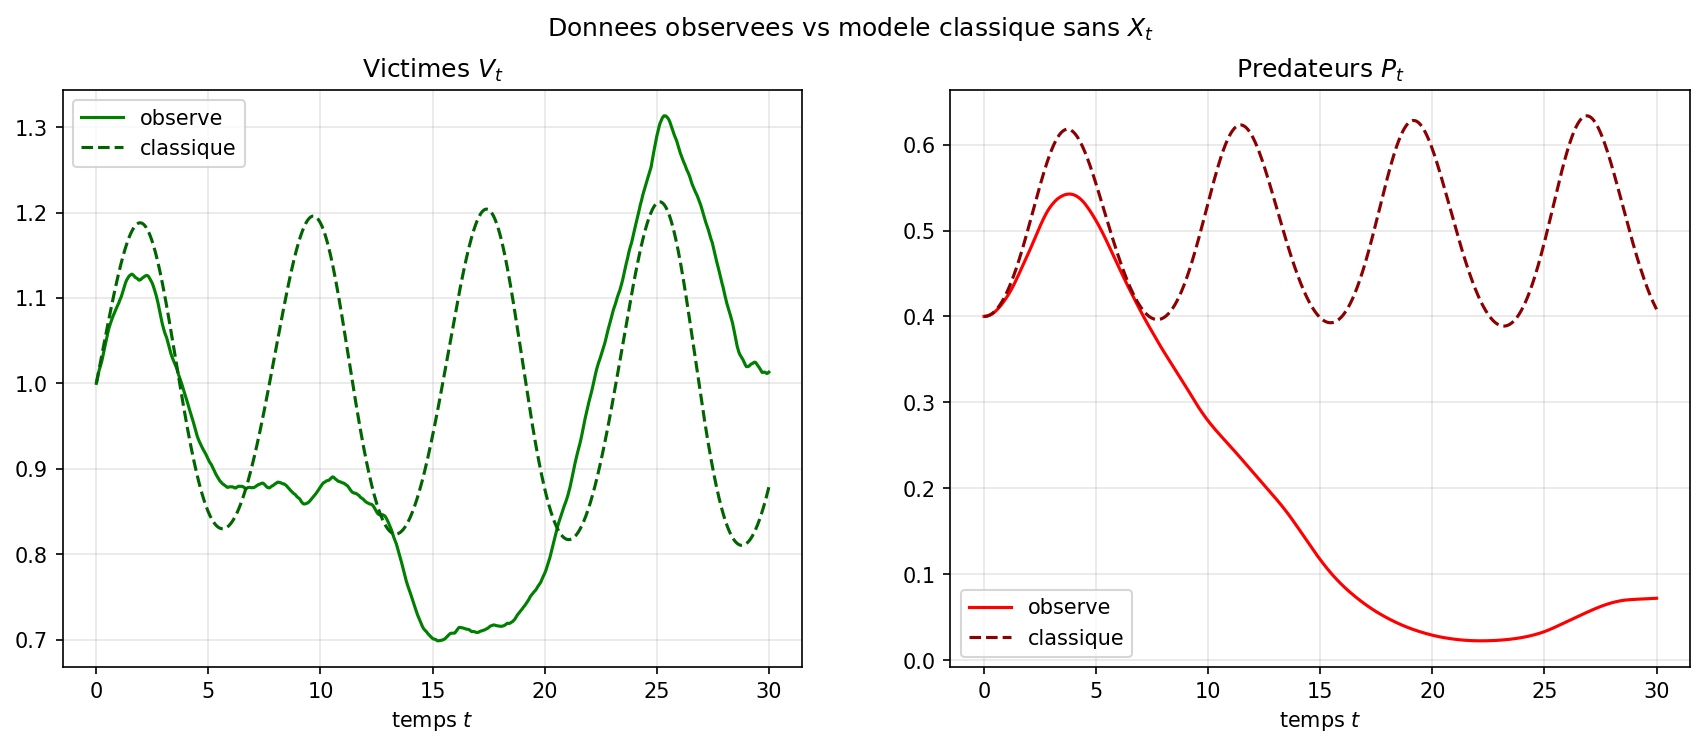
\includegraphics[width=\textwidth]{virus4_comparaison.png}
  \caption{Comparaison entre les données observées (trait plein) et le modèle de Lotka-Volterra classique sans $X_t$ (tirets), pour les victimes (gauche) et les prédateurs (droite).}
  \label{fig:comparaison}
\end{figure}

La comparaison nous a semblé parlante. Le modèle classique produit des oscillations régulières et entretenues où les deux populations tournent indéfiniment autour de leur point d'équilibre et où le portrait de phase serait une courbe fermée bien nette. Les données observées partent dans la même direction au tout début mais s'en écartent franchement ensuite. La population de prédateurs ne semble notamment pas ré-osciller puisqu'elle s'effondre progressivement et reste très basse alors que le modèle classique la voit remonter à chaque cycle.

Nous en avons retiré l'impression que le terme de virus $X_t$ ne se contente pas d'ajouter un petit bruit autour de la trajectoire classique mais qu'il modifie la dynamique d'ensemble et casse la périodicité. C'est sur ce comportement que nous avons choisi d'appuyer la modélisation de $(X_t)$ dans la suite.

\subsection*{Reconstruction du virus $X_t$}

Ces premières observations restent qualitatives. Pour aller plus loin il nous a semblé qu'il fallait regarder directement le virus $X_t$, qui porte l'information utile sur la perturbation. Or l'équation des proies le fait apparaître explicitement, si bien qu'il suffit de la discrétiser pour l'en extraire. En remplaçant $dV_t$ par la différence $V_i - V_{i-1}$ et en évaluant le membre de droite au début du pas, on obtient

\begin{equation}\label{eq:disc}
  V_i - V_{i-1} \approx V_{i-1}\left(\tfrac{2}{3} - \tfrac{4}{3}P_{i-1} + X_{i-1}\right)dt.
\end{equation}

Tous les autres termes étant connus, il ne reste qu'à isoler le virus.

\begin{equation}\label{eq:xrec}
  X_{i-1} \approx \frac{V_i - V_{i-1}}{V_{i-1}\,dt} - \tfrac{2}{3} + \tfrac{4}{3}P_{i-1}.
\end{equation}

Cette reconstruction est entièrement déterministe puisqu'elle ne fait qu'inverser le schéma, sans aucune hypothèse de modèle. La figure~\ref{fig:xt} montre le virus reconstruit et ses différences.

\begin{figure}[ht]
  \centering
  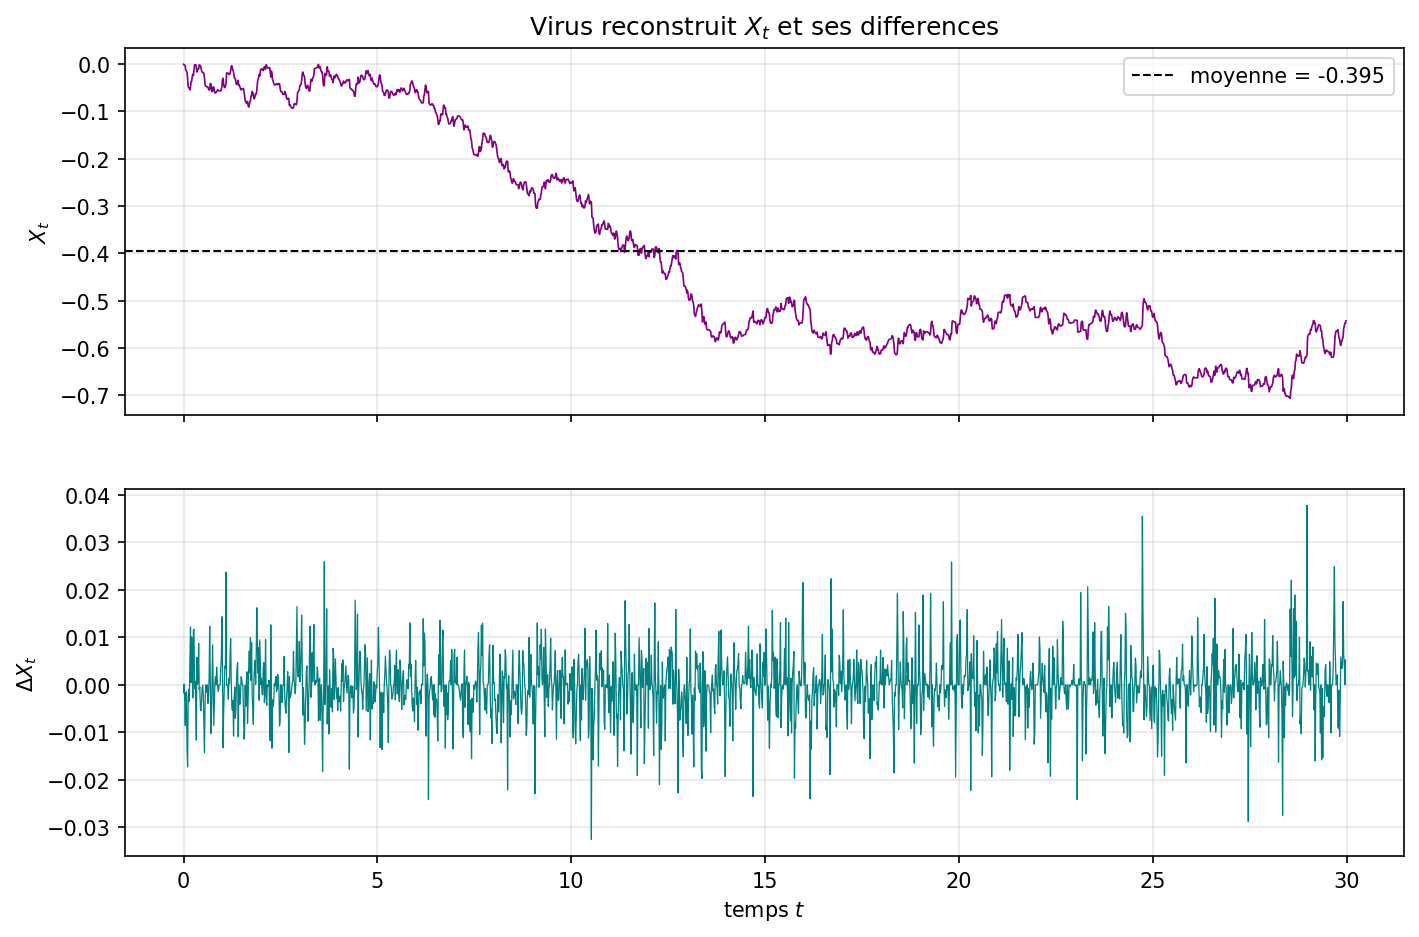
\includegraphics[width=0.8\textwidth]{virus4_Xt.png}
  \caption{En haut, le virus reconstruit $X_t$, de moyenne empirique $\approx -0{,}40$ et d'écart-type $\approx 0{,}23$. En bas, ses différences $\Delta X_t = X_{t+dt} - X_t$.}
  \label{fig:xt}
\end{figure}

Le virus reconstruit est en moyenne nettement négatif. En revanche, le graphe des différences ne nous apprend pas grand-chose à lui seul.

\begin{figure}[h]
  \centering
  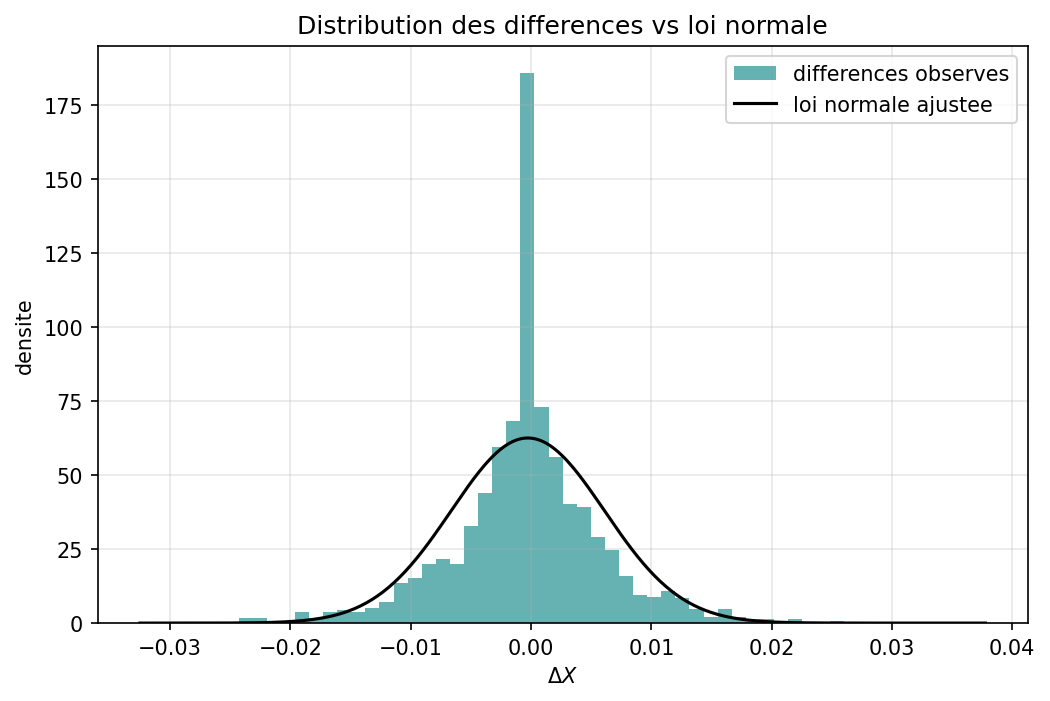
\includegraphics[width=0.65\textwidth]{virus4_dXt_hist.png}
  \caption{Distribution des différences $\Delta X_t$ comparée à une loi normale de mêmes moyenne et écart-type. La forme est plus piquée et à queues plus lourdes qu'une gaussienne.}
  \label{fig:hist}
\end{figure}

Toutefois, dans les processus stochastiques, les différences jouent un rôle central, et une première idée naturelle est de vérifier si elles sont gaussiennes. La distribution observée s'écarte nettement de la loi normale calée sur la moyenne et l'écart-type empiriques des différences.

Un test de Kolmogorov-Smirnov donne ici une p-value de l'ordre de $6\cdot10^{-14}$, largement inférieure à $0{,}05$. \textbf{À priori, l'hypothèse d'une distribution gaussienne des différences n'est pas retenue.}

\subsection*{Un modèle du cours pour $X_t$ ?}

Une première idée naturelle est de passer en revue les modèles vus en cours pour juger de leur pertinence. Le tableau~\ref{tab:modeles} indique, pour chaque modèle écarté, la raison de l'écarter. Les modèles que rien ne permet d'écarter restent simplement en lice.

\begin{table}[ht]
  \centering
  \resizebox{\textwidth}{!}{%
  \begin{tabular}{llcl}
    \hline
    Modèle & Caractéristiques & Retenu & Justification \\
    \hline
    Brownien avec dérive & tendance linéaire & $\checkmark$ &  \\
    Brownien géométrique & reste de signe constant & $\times$ & $X_t$ devient négatif \\
    Pont brownien & épinglé aux deux bords & $\times$ & $X_t$ ne revient pas au départ \\
    Brownien intégral & trajectoire très lisse & $\times$ & différences trop bruitées \\
    Ornstein-Uhlenbeck & retour à la moyenne & $\checkmark$ &  \\
    Verhulst (logistique) & saturation, population positive & $\times$ & virus négatif mal décrit \\
    \hline
  \end{tabular}%
  }
  \caption{Modèles vus en cours et leur pertinence pour $(X_t)$. On ne justifie que les rejets ; les modèles retenus sont simplement ceux que rien ne permet d'écarter à ce stade.}
  \label{tab:modeles}
\end{table}

\subsection*{Tester un modèle par ses résidus}

Deux candidats passent ce premier filtre, le brownien avec dérive et l'Ornstein-Uhlenbeck. Sur une fenêtre aussi courte nous ne distinguons d'ailleurs pas à l'œil une dérive lente d'un retour à la moyenne. Ils s'écrivent respectivement

\begin{equation}\label{eq:modeles}
  dX_t = \nu\,dt + \sigma\,dB_t \qquad \text{et} \qquad dX_t = \theta(\mu - X_t)\,dt + \sigma\,dB_t,
\end{equation}

et se mettent tous deux sous la forme générale $dX_t = a(X_t)\,dt + \sigma\,dB_t$, où $a(X_t)$ désigne la dérive du modèle, égale à la constante $\nu$ pour le premier et à $\theta(\mu - X_t)$ pour le second. Une fois cette dérive retirée, il ne doit rester qu'un bruit brownien, si bien que le résidu standardisé

\begin{equation}\label{eq:residu}
  \varepsilon_i = \frac{\Delta X_i - a(X_i)\,dt}{\sigma\sqrt{dt}} = \frac{\Delta B_i}{\sqrt{dt}}
\end{equation}

n'est qu'un incrément de mouvement brownien ramené à l'échelle $\sqrt{dt}$. Comme un tel incrément suit $\mathcal N(0,dt)$, le résidu doit suivre une loi normale centrée réduite $\mathcal N(0,1)$, et les résidus successifs doivent être indépendants. Un modèle pertinent devrait donc d'abord passer ce test des résidus, qui porte sur leur loi et sur leur indépendance.

\subsection*{Test du brownien avec dérive}

En discrétisant son équation, $\Delta X_i = \nu\,dt + \sigma\,\Delta B_i$. La moyenne des différences donne $\nu$, et comme l'incrément $\Delta B_i$ est d'écart-type $\sqrt{dt}$, l'écart-type des différences vaut $\sigma\sqrt{dt}$, ce qui donne $\sigma$ :

\begin{center}
  $\nu = \overline{\Delta X}/dt \approx -0{,}02, \qquad \sigma = \mathrm{std}(\Delta X)/\sqrt{dt} \approx 0{,}05.$
\end{center}

La dérive étant constante, les résidus $\varepsilon_i = (\Delta X_i - \nu\,dt)/(\sigma\sqrt{dt})$ ne sont que les différences recentrées et réduites. La figure~\ref{fig:res-derive} compare leur histogramme à la loi $\mathcal N(0,1)$ attendue.

\begin{figure}[ht]
  \centering
  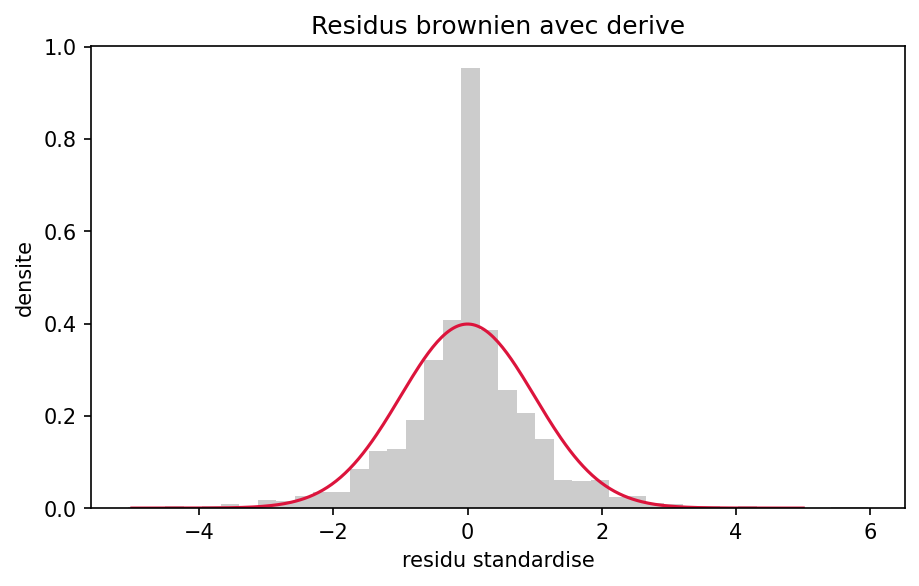
\includegraphics[width=0.5\textwidth]{virus4_residus_derive.png}
  \caption{Histogramme des résidus standardisés du brownien avec dérive, comparé à la loi normale centrée réduite.}
  \label{fig:res-derive}
\end{figure}

Le test de Kolmogorov-Smirnov contre $\mathcal N(0,1)$ donne une p-value de l'ordre de $10^{-14}$, et les résidus consécutifs gardent une corrélation de l'ordre de $0{,}26$, loin de l'indépendance d'un bruit brownien.

\textbf{À priori, le brownien avec dérive n'est pas retenu.}

\subsection*{Test de l'Ornstein-Uhlenbeck}

En discrétisant son équation, on obtient

\begin{equation}\label{eq:ou-disc}
  \Delta X_i \approx \theta\mu\,dt - \theta\,dt\,X_i + \sigma\,\Delta B_i,
\end{equation}

une relation linéaire entre $\Delta X_i$ et $X_i$. Sa pente vaut $-\theta\,dt$ et son ordonnée à l'origine $\theta\mu\,dt$, ce qui donne $\theta$ puis $\mu$, tandis que l'écart-type des résidus de la régression donne $\sigma\sqrt{dt}$. On trouve :

\begin{center}
  $\theta \approx 0{,}07, \qquad \mu \approx -0{,}66, \qquad \sigma \approx 0{,}05.$
\end{center}

Les résidus standardisés $\varepsilon_i = (\Delta X_i - \theta(\mu - X_i)\,dt)/(\sigma\sqrt{dt})$ devraient de même suivre $\mathcal N(0,1)$. Le terme de rappel retiré étant minime, leur histogramme reste celui de la dérive (figure~\ref{fig:res-ou}).

\begin{figure}[ht]
  \centering
  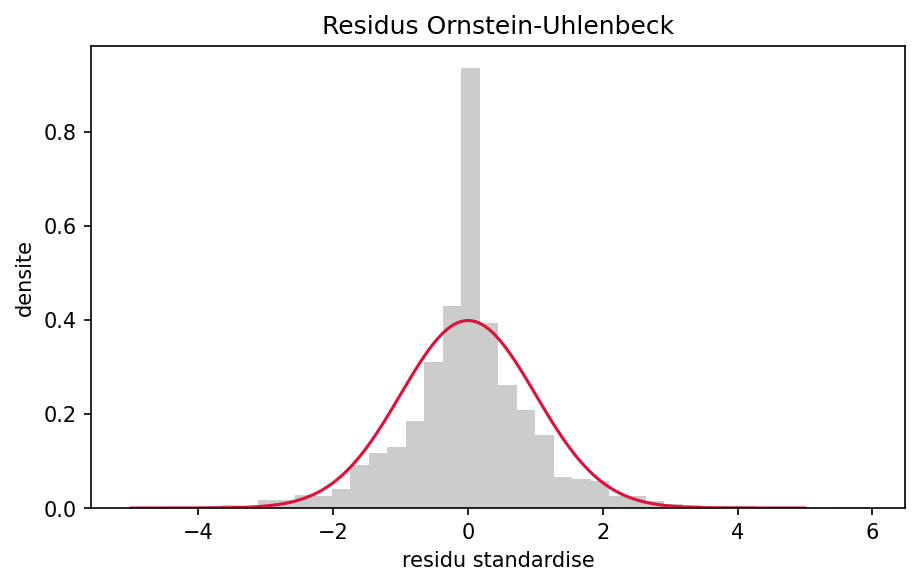
\includegraphics[width=0.5\textwidth]{virus4_residus_ou.png}
  \caption{Histogramme des résidus standardisés de l'Ornstein-Uhlenbeck, comparé à la loi normale centrée réduite.}
  \label{fig:res-ou}
\end{figure}

Le test de Kolmogorov-Smirnov contre $\mathcal N(0,1)$ donne là aussi une p-value de l'ordre de $10^{-14}$, et la corrélation entre résidus consécutifs reste de l'ordre de $0{,}26$.

\textbf{À priori, l'Ornstein-Uhlenbeck n'est pas retenu.}

\subsection*{Bilan}

Les deux candidats sont écartés pour la même raison. Tous deux reposent sur un bruit brownien, donc sur des résidus gaussiens et indépendants, alors que ceux du virus reconstruit présentent deux défauts bien distincts. Ils restent corrélés d'un pas au suivant, ce qui trahit une mémoire, et ils s'écartent nettement d'une loi normale par des queues plus lourdes. Plutôt que d'abandonner d'emblée le cadre des EDS, il nous a semblé plus instructif de corriger ces deux défauts l'un après l'autre.

\subsection*{Un bruit coloré à mémoire}

Le premier défaut à corriger est la mémoire. Une idée a été de renoncer au bruit blanc et de donner au bruit lui-même une corrélation d'un pas au suivant, c'est-à-dire de le décrire par un Ornstein-Uhlenbeck. En discrétisant un tel bruit $dE_t = -\theta E_t\,dt + s\,dB_t$, on obtient $E_i = (1 - \theta\,dt)\,E_{i-1} + s\,\Delta B_i$, soit une relation autorégressive d'ordre un sur les résidus

\begin{equation}\label{eq:ar1}
  \varepsilon_i = \phi\,\varepsilon_{i-1} + \eta_i,
\end{equation}

où $\phi = 1 - \theta\,dt$ porte la mémoire tandis que les innovations $\eta_i = s\,\Delta B_i$ doivent retrouver le statut d'un bruit blanc gaussien. Tester ce modèle revient à régresser les résidus de l'Ornstein-Uhlenbeck sur leur passé pour estimer $\phi$, puis à vérifier que les innovations $\eta_i = \varepsilon_i - \phi\,\varepsilon_{i-1}$ sont indépendantes et gaussiennes.

La régression donne directement la mémoire et nous standardisons ensuite les innovations pour les comparer à $\mathcal N(0,1)$.

\begin{center}
  $\phi \approx 0{,}26.$
\end{center}

La corrélation entre innovations consécutives tombe à $\approx 0{,}02$ alors que les résidus de départ en gardaient $\approx 0{,}26$, si bien que la mémoire est effectivement captée par le terme autorégressif. La loi, en revanche, ne s'améliore pas. Le test de Kolmogorov-Smirnov des innovations contre $\mathcal N(0,1)$ donne une p-value de l'ordre de $4\cdot10^{-14}$, largement inférieure à $0{,}05$ (figure~\ref{fig:res-colore}).

\begin{figure}[ht]
  \centering
  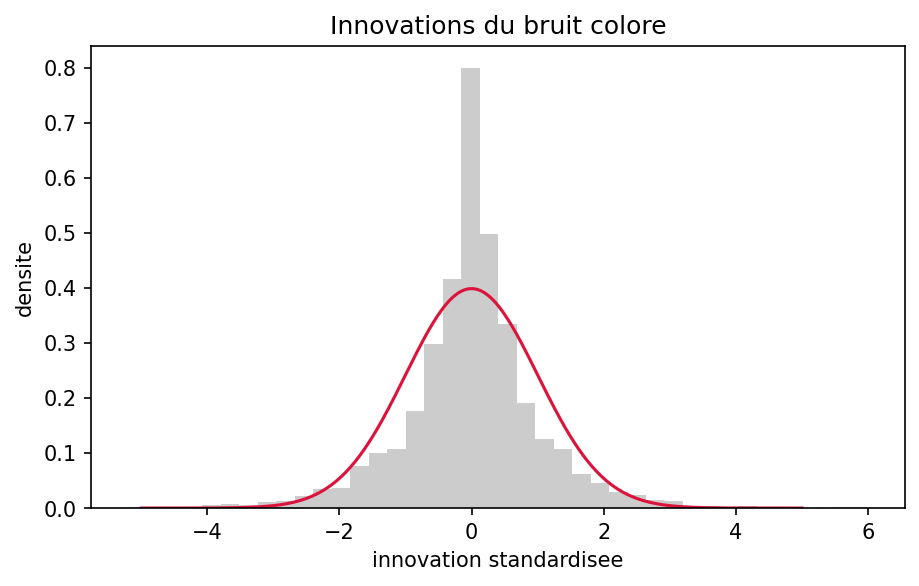
\includegraphics[width=0.5\textwidth]{virus4_residus_colore.png}
  \caption{Histogramme des innovations standardisées du bruit coloré, comparé à la loi normale centrée réduite. Le terme autorégressif retire la mémoire mais les queues restent trop lourdes.}
  \label{fig:res-colore}
\end{figure}

\textbf{À priori, l'indépendance est rétablie tandis que l'hypothèse d'innovations gaussiennes n'est pas retenue.}

\subsection*{La loi des innovations}

La mémoire étant captée par le terme autorégressif, il restait à corriger la loi des innovations. Leur histogramme reste plus piqué et à queues plus lourdes qu'une gaussienne, ce qui nous a conduits à tester une loi de Student. Une telle loi sort du cadre brownien strict puisque les incréments d'un mouvement brownien y sont gaussiens par construction, mais son nombre de degrés de liberté $\nu$ règle l'épaisseur des queues et permet de les ajuster.

Nous avons ajusté une loi de Student aux innovations par maximum de vraisemblance puis comparé cet ajustement à la gaussienne, dans les deux cas par un test de Kolmogorov-Smirnov.

\begin{center}
  $\nu \approx 2{,}4.$
\end{center}

Le test contre la Student donne une p-value de l'ordre de $2\cdot10^{-2}$, contre $4\cdot10^{-14}$ pour la gaussienne (figure~\ref{fig:student}).

\begin{figure}[ht]
  \centering
  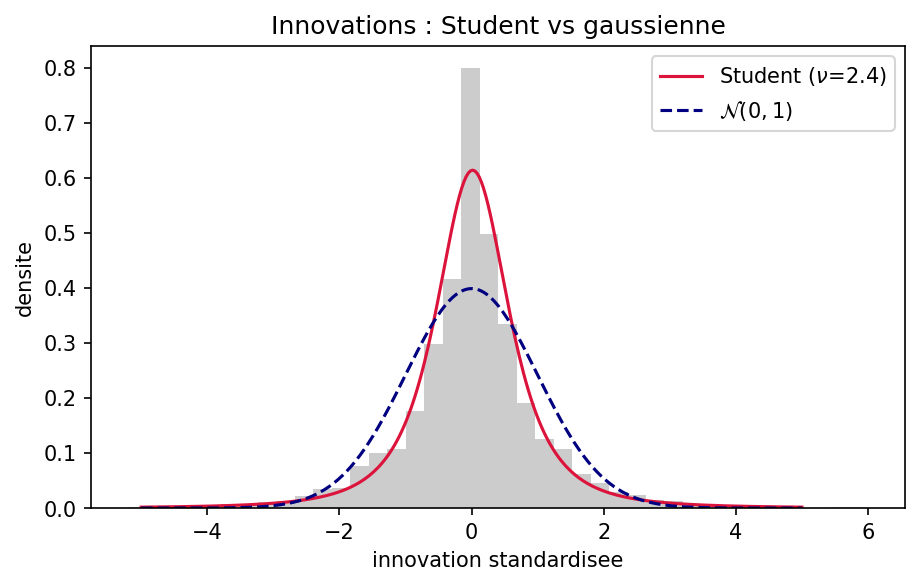
\includegraphics[width=0.5\textwidth]{virus4_innovations_student.png}
  \caption{Innovations standardisées comparées à la loi de Student ajustée ($\nu \approx 2{,}4$) et à la loi normale centrée réduite. La Student épouse bien mieux les queues lourdes.}
  \label{fig:student}
\end{figure}

La p-value remonte de douze ordres de grandeur mais reste, à $\approx 0{,}02$, en dessous de $0{,}05$. \textbf{À priori, l'hypothèse d'innovations exactement de Student n'est pas retenue, même si cette loi décrit nettement mieux les innovations que la gaussienne.}

\section*{Question 2 — Probabilités d'extinction}

Une fois un modèle pour $X_t$ en main, nous nous sommes demandé avec quelle probabilité une population finit par s'éteindre, c'est-à-dire passe sous le seuil de densité $0{,}01$ au cours de l'intervalle $[0,\tau]$. Aucune de nos deux lois d'innovations n'ayant été formellement retenue, nous sommes partis du modèle qui capte le mieux la dynamique, soit l'Ornstein-Uhlenbeck dont le bruit est coloré par la mémoire $\phi$, et nous l'avons injecté dans le système $(V,P)$ pour estimer ces probabilités par Monte-Carlo.

\subsection*{Méthode}

Nous simulons $M$ trajectoires indépendantes du système complet. Le virus $X_t$ suit l'Ornstein-Uhlenbeck calibré plus haut dont le bruit obéit à la récurrence autorégressive~\eqref{eq:ar1}, tandis que les populations $(V,P)$ sont intégrées par un schéma d'Euler sur la même grille de temps que les données. Une trajectoire est comptée comme une extinction pour une population dès que sa densité passe sous $0{,}01$ en un point de $[0,\tau]$. Chaque trajectoire est alors une épreuve de Bernoulli si bien que le nombre d'extinctions parmi les $M$ tirages suit une loi binomiale $\mathcal B(M,p)$. La loi des grands nombres assure que la proportion observée estime $p$, et le théorème central limite donne un intervalle de confiance à $95\,\%$ de demi-largeur $1{,}96\sqrt{p(1-p)/M}$.

\subsection*{Résultats}

Avec $M = 10\,000$ trajectoires, les probabilités d'extinction estimées sont très contrastées d'une population à l'autre.

\begin{center}
  victimes : $p \approx 0{,}004$ \quad (IC$_{95}$ $[0{,}003\,;\,0{,}005]$) \\[0.3em]
  prédateurs : $p \approx 0{,}44$ \quad (IC$_{95}$ $[0{,}43\,;\,0{,}45]$)
\end{center}

La figure~\ref{fig:conv} suit l'estimée cumulée et sa bande de confiance au fil des simulations, qui se resserre nettement et confirme la convergence. La figure~\ref{fig:traj} illustre le mécanisme sur quelques trajectoires simulées, où l'on voit les prédateurs frôler ou franchir le seuil bien plus souvent que les victimes.

\begin{figure}[ht]
  \centering
  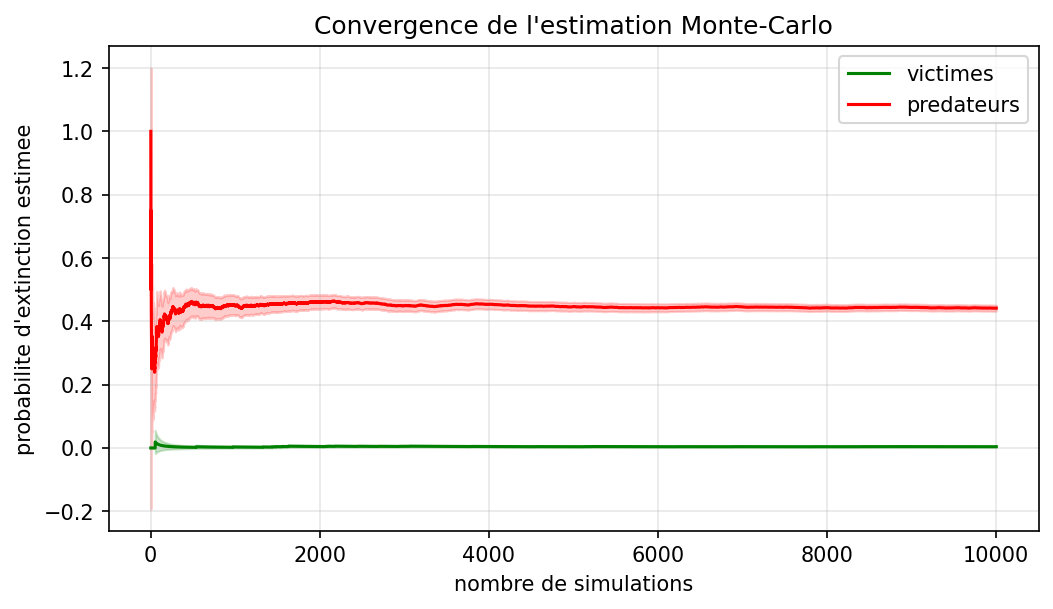
\includegraphics[width=0.7\textwidth]{virus4_extinction_convergence.png}
  \caption{Convergence des probabilités d'extinction estimées en fonction du nombre de simulations, avec leur bande de confiance à $95\,\%$.}
  \label{fig:conv}
\end{figure}

\begin{figure}[ht]
  \centering
  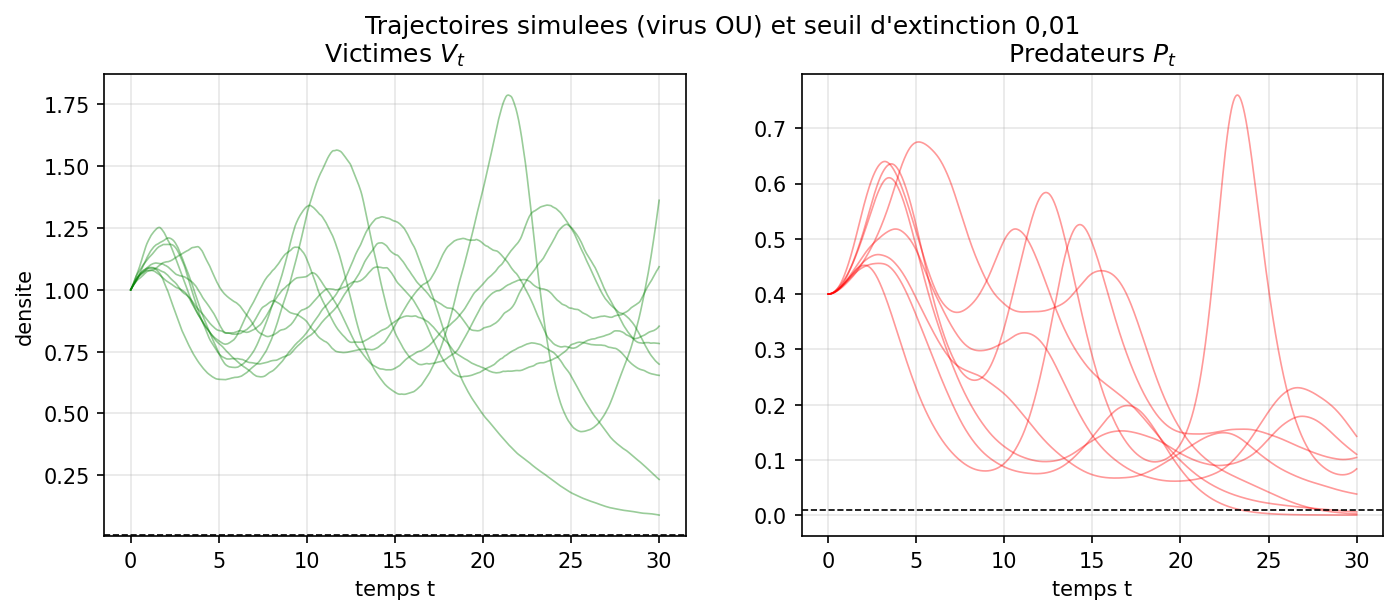
\includegraphics[width=\textwidth]{virus4_extinction_trajectoires.png}
  \caption{Quelques trajectoires simulées des victimes (gauche) et des prédateurs (droite) sous le bruit coloré, avec le seuil d'extinction $0{,}01$ en tirets.}
  \label{fig:traj}
\end{figure}

Les prédateurs sont donc bien plus exposés que les victimes, ce qui rejoint le comportement déjà lu sur les données (figure~\ref{fig:series}) où ils s'effondrent durablement alors que les victimes continuent d'osciller. Une moyenne $m$ négative du virus abaisse l'équilibre des prédateurs via la relation~\eqref{eq:equilibre} et les rapproche du seuil, tandis que les victimes restent à des densités confortables.

\subsection*{Robustesse au choix de la loi}

Puisque ni la loi gaussienne ni la Student n'ont été retenues, il nous a semblé prudent de vérifier que ces probabilités ne dépendent pas du choix laissé en suspens. Nous avons rejoué les simulations à mémoire $\phi$ identique en ne changeant que la loi des innovations, gaussienne d'un côté et Student standardisée de l'autre.

\begin{center}
  bruit gaussien : victimes $0{,}004$, prédateurs $0{,}44$ \\[0.3em]
  bruit Student : victimes $0{,}006$, prédateurs $0{,}40$
\end{center}

\begin{figure}[ht]
  \centering
  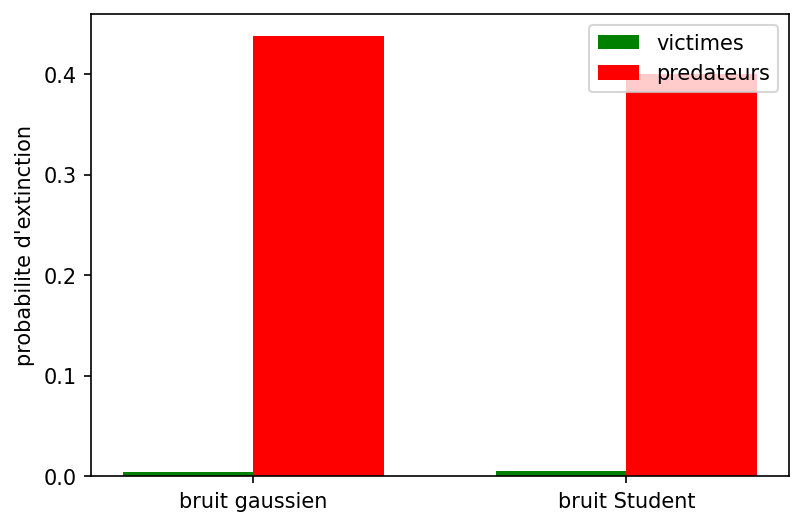
\includegraphics[width=0.55\textwidth]{virus4_extinction_comparaison.png}
  \caption{Probabilités d'extinction des deux populations selon que le bruit coloré porte des innovations gaussiennes ou de Student.}
  \label{fig:comp}
\end{figure}

Les ordres de grandeur ne bougent pas d'une loi à l'autre. \textbf{La conclusion d'un risque fort pour les prédateurs et quasi nul pour les victimes est donc robuste au choix de la loi des innovations, pourtant non tranché.}

\end{document}
